%
% LaTeX template for prepartion of submissions to PLDI'16
%
% Requires temporary version of sigplanconf style file provided on
% PLDI'16 web site.
% 
%\documentclass[format=sigconf]{acmart}
%\documentclass[conference]{IEEEtran}
%\documentclass[elsarticle]
%\documentclass[preprint,12pt,authoryear]{elsarticle}
%\documentclass[preprint,12pt]{elsarticle}
\documentclass[sigconf]{acmart}


% \documentclass[pldi-cameraready]{sigplanconf-pldi16}

%
% the following standard packages may be helpful, but are not required
%
%\usepackage{SIunits}            % typset units correctly
%\usepackage{courier}            % standard fixed width font
%\usepackage[scaled]{helvet} % see www.ctan.org/get/macros/latex/required/psnfss/psnfss2e.pdf
\usepackage{url}                  % format URLs
\usepackage{listings}          % format code
\usepackage{enumitem}      % adjust spacing in enums
\usepackage{graphicx}
\usepackage{amsmath}
\usepackage{mathtools}
%\usepackage{caption}
\usepackage{subcaption}
\usepackage{code}
%\usepackage[colorlinks=true,allcolors=blue,breaklinks,draft=false]{hyperref}   % hyperlinks, including DOIs and URLs in bibliography
% known bug: http://tex.stackexchange.com/questions/1522/pdfendlink-ended-up-in-different-nesting-level-than-pdfstartlink
%\newcommand{\doi}[1]{doi:~\href{http://dx.doi.org/#1}{\Hurl{#1}}}   % print a hyperlinked DOI


%\numberofauthors{2}

%\alignauthor
%Josie Holmes\\
%\alignauthor 
%Alex Groce\\
%      \affaddr{School of Informatics, Computing \& Cyber Systems}\\
%       \affaddr{Northern Arizona University
%}

%\setcopyright{rightsretained}
%\setcopyright{usgov}
%\setcopyright{usgovmixed}
%\setcopyright{cagov}
%\setcopyright{cagovmixed}


% DOI
%\acmDOI{10.475/123_4}

% ISBN
%\acmISBN{123-4567-24-567/08/06}

%Conference
%\acmConference[ISSTA'17]{International Symposium on Software Testing
 % and Analysis}{July 2017}{Santa Barbara, California, USA}
%\acmYear{2017}
%\copyrightyear{2017}

%\newcommand{\comment}[1]{}

\begin{document}

%\begin{frontmatter}

\title{Using Differential Mutation Analysis to Compare and Improve
  Static Analysis Tools}


%\author{
%\IEEEauthorblockN{Alex Groce}
%\IEEEauthorblockA{School of Informatics, Computing \& Cyber Systems\\
%Northern Arizona University\\
%Email: agroce@gmail.com}
%\and
%\IEEEauthorblockN{Josie Holmes}
%\IEEEauthorblockA{School of Informatics, Computing \& Cyber Systems\\
%Northern Arizona University\\
%Email: josie.holmes@nau.edu}}

%\author{Alex Groce}
%\ead{agroce@gmail.com}
%\ead{https://agroce.github.io}
%\address{School of Informatics, Computing \& Cyber Systems\\Northern
%  Arizona University}
%\author{Josie Holmes}
%\ead{josie.holmes@nau.edu}
%\address{School of Informatics, Computing \& Cyber Systems\\Northern
%  Arizona University}

%
% any author declaration will be ignored  when using 'pldi' option (for double blind review)
%

%\authorinfo{Person 1 \and Person 2}
%{\makebox{A Department} \\
%\makebox{A University}  \\
%\makebox{A Place, AS 12345}}
%{\{person1,person2\}@cs.auniv.edu}

%\begin{CCSXML}
%<ccs2012>
%<concept>
%<concept_id>10011007.10010940.10010992.10010998.10011001</concept_id>
%<concept_desc>Software and its engineering~Dynamic analysis</concept_desc>
%<concept_significance>500</concept_significance>
%</concept>
%<concept>
%<concept_id>10011007.10011074.10011099.10011102.10011103</concept_id>
%<concept_desc>Software and its engineering~Software testing and debugging</concept_desc>
%<concept_significance>500</concept_significance>
%</concept>
%</ccs2012>
%\end{CCSXML}

%\ccsdesc[500]{Software and its engineering~Dynamic analysis}
%\ccsdesc[500]{Software and its engineering~Software testing and debugging}

%\keywords{mutants, distance metrics, fault identification/localization}


\begin{abstract}
Many programming languages offer multiple static analysis tools that offer to detect faults in code without executing it.  Understanding the strengths and weaknesses of tools, and performing direct comparisons of their effectiveness is difficult; it usually involves either manual examination of differing warnings on real code, or the bias-prone construction of artificial test cases.  In practice, comparisons tend to be limited to superficial, anecdotal discussions in the informal literature (e.g., blog posts by software developers), or purely research-community-oriented evaluations made by the authors of new tools seeking to publish their results.  This paper proposes a novel automated approach to comparing static analysis tools, based on producing \emph{mutants} of real code, and comparing mutation detection rates for tools to their warning rates on the original code.  In addition to making tool differences quantitatively observable without extensive manual effort, this approach offers a new way to detect and fix omissions in a static analysis tool's set of detectors.  We present an extensive comparison of three well-known Solidity smart contract static analysis tools, and show how using an automatic prioritization of our results allowed us to add three effective new detectors as an open source contribution to the best of the tools.  We also evaluate popular Java and Python static analysis tools and discuss their strengths and weaknesses.
\end{abstract}

\maketitle 



%\begin{keyword}
%determinism, flaky tests, library testing, random testing,
%specification mechanisms, test case reduction
%\end{keyword}

%\end{frontmatter}

\section{Introduction}

Static analysis of code is one of the most effective ways to avoid defects in software, and, when security is a concern, is essential.  Static analysis can find problems that are extremely hard to detect by testing, when the inputs triggering a bug are hard to find.  Static analysis is also often more efficient than testing; a bug that takes a fuzzer days to find may be immediately identified.
Users of static analysis tools often wonder which of multiple tools available for a language are most effective, and how much tools overlap in their results.  Tools often find substantially different bugs, making it important to use multiple tools \cite{AllBugs}.  However, given the high cost of examing results, if a tool provides only marginal novelty, it may not be worth using, especially if it has a high false-positive rate.  Developers of static analysis tools also want to be able to compare their tools to other tools, in order to see what detection patterns or precision/soundness trade-offs they might want to imitate.  Unfortunately, comparing static analysis tools in these ways is hard, and would seem to require vast manual effort to inspect findings and determine ground truth on a scale that would provide statistical confidence.

Differential testing \cite{Differential,ICSEDiff,csmith} is a popular approach to comparing multiple software systems offering similar functionality, but the wide divergence of possible trade-offs, analysis focuses, and the prevalence of false positives in almost all analysis results makes na\"ive differential testing not applicable to static analysis tools \cite{regehrRandom}.
Mutation analysis\cite{jia2011analysis,demillo1978hints,budd1980theoretical} uses small syntactic changes to a program to introduce synthetic ``faults,'' under the assumption that if the original version of a program is mostly correct, such changes will often introduce a fault.  For the most part, mutation analysis has been used to evaluate test suites by computing a mutation score, the fraction of mutants the suite detects, or ``kills''.  
Groce et al. \cite{groce2015verified,groce2018verified} proposed examining individual mutants that survive a rigorous testing and verification effort to detect and correct weaknesses in testing, and found bugs in a heavily-tested module of the Linux kernel \cite{mutKernel} and a widely used Python file system.  Recently, mutation analysis has been adopted in industrial settings, though not for actual examination of all surviving mutants \cite{MutGoogle,ivankovic2018industrial}.

Combining a differential approach and mutation analysis offers a novel way to compare static analysis tools, one useful to users wishing to select a good tool or set of tools, to researchers interested in the impact of precision/soundness trade-offs or different intermediate languages, and to developers of static analysis tools hoping to improve their tools.

%\subsection{Differential Mutation Analysis}

We can say that a static analysis tool kills a mutant when the \emph{number of warnings or errors}, which we call \emph{findings}, \emph{increases with mutation}.  In order to make this definition useful, we ignore informational or optimization related warnings (e.g., if a mutant is merely \emph{stylistically} suboptimal this is not ``finding a fault''). That is, a mutant is killed when a tool ``finds more (unique) bugs'' for the mutated code than for the un-mutated code.  This difference may be most easily interpreted when the original code produces no findings; we call such code \emph{clean} (by analogy with Chekam et al.'s notion \cite{CleanProgram}). For non-clean code, a tool conceivably could detect the mutant, but only change a previously generated finding, not add an additional finding.  However, even for non-clean code, \emph{most detected mutants should produce a new warning}.  We count findings, rather than consider their location or type, because some mutants cause a fault at a far-removed location.  Forcing tools to produce an \emph{additonal} warning is a conservative and automatable estimate of mutant detection.

The value of the differential comparison lies in a few key points.  First, this is a measure that does not reward a tool that produces too many false positives.  The tool cannot simply flag all code as having a problem or it will perform poorly at the task of \emph{distinguishing} the mutated code from non-mutated, and presumably at least \emph{more} correct, code.  Based on verification and testing uses of mutation, it is safe to say that usually at minimum 40\%, often 50-60\%, and frequently up to 80\%+ \cite{mutKernel,groce2018verified,le2014mucheck}, of mutants are not semantically equivalent to the original code \cite{TCE,impactEquiv,smith2009should}, so the task presented to a static analysis tool is simply the core functionality of static analysis: \emph{to distinguish faulty from correct code without execution}.  Obviously, many faults cannot be identified statically without a complete specification, or without unreasonable analysis cost and precision, but the measure of performance here is \emph{relative} to other tools applied to the same code; this is primarily a \emph{differential} approach.  While many mutants cannot be detected statically, the ones that \emph{are} tend to be \emph{true positives}: \emph{if} they were real code changes, they would be faults.  \emph{We manually confirmed that for a large portion of the detected mutants in our experiments, the changes were indeed ones that would be real faults if present in the code.}

Second, and critically, this is an \emph{automatable} method that can provide an evaluation of static analysis tools over a large number of target source code files, without requiring human effort to classify results as real bugs or false positives.  It is not clear that any other fully automatic method is competitively meaningful; it is possible that methods based on code changes from version control provide some of the same benefits, but these require classification of changes into bug-fixes and non-bug-fixes, and of course require version control history.  Also, history-based methods will be biased towards precisely those faults humans or tools already in use were able to detect and fix.  Rather than the hundreds \cite{just2014defects4j} or at most few thousand of faults \cite{BugSwarm} in benchmark defect sets, our approach enables the use of \emph{many tens of thousands} of hypothetical faults.

It is the combination of differential comparison and mutation that is key.  Differential comparison of tools, as noted above, is not really meaningful, without additional effort; na\"ive methods simply will not work \cite{regehrRandom}.  Consider a comparison of the number of findings between two tools over a single program, or over a large set of programs.  If one tool emits more warnings and errors than another, it may mean that the tool is more effective at finding bugs; but it may also mean that it has a higher false positive rate.  Without human examination of the individual findings, it is impossible to be sure.  Using mutants, however, provides a foreground to compare to this background.  In particular, for a large set of programs, the most informative result will be when 1) tool A reports fewer findings on average than tool B over the un-mutated programs but 2) tool A also detects more mutants.  This is strong evidence that A is simply better all-around than B; it likely has a lower false positive rate \emph{and} a lower false negative rate, since it is hard to construct another plausible explanation for reporting \emph{fewer} findings on un-mutated code while still detecting \emph{more} mutants.  Our method (see the \emph{mutant ratio} defined below) provides a quantitative measure of this insight.

\begin{figure}
  \centering
  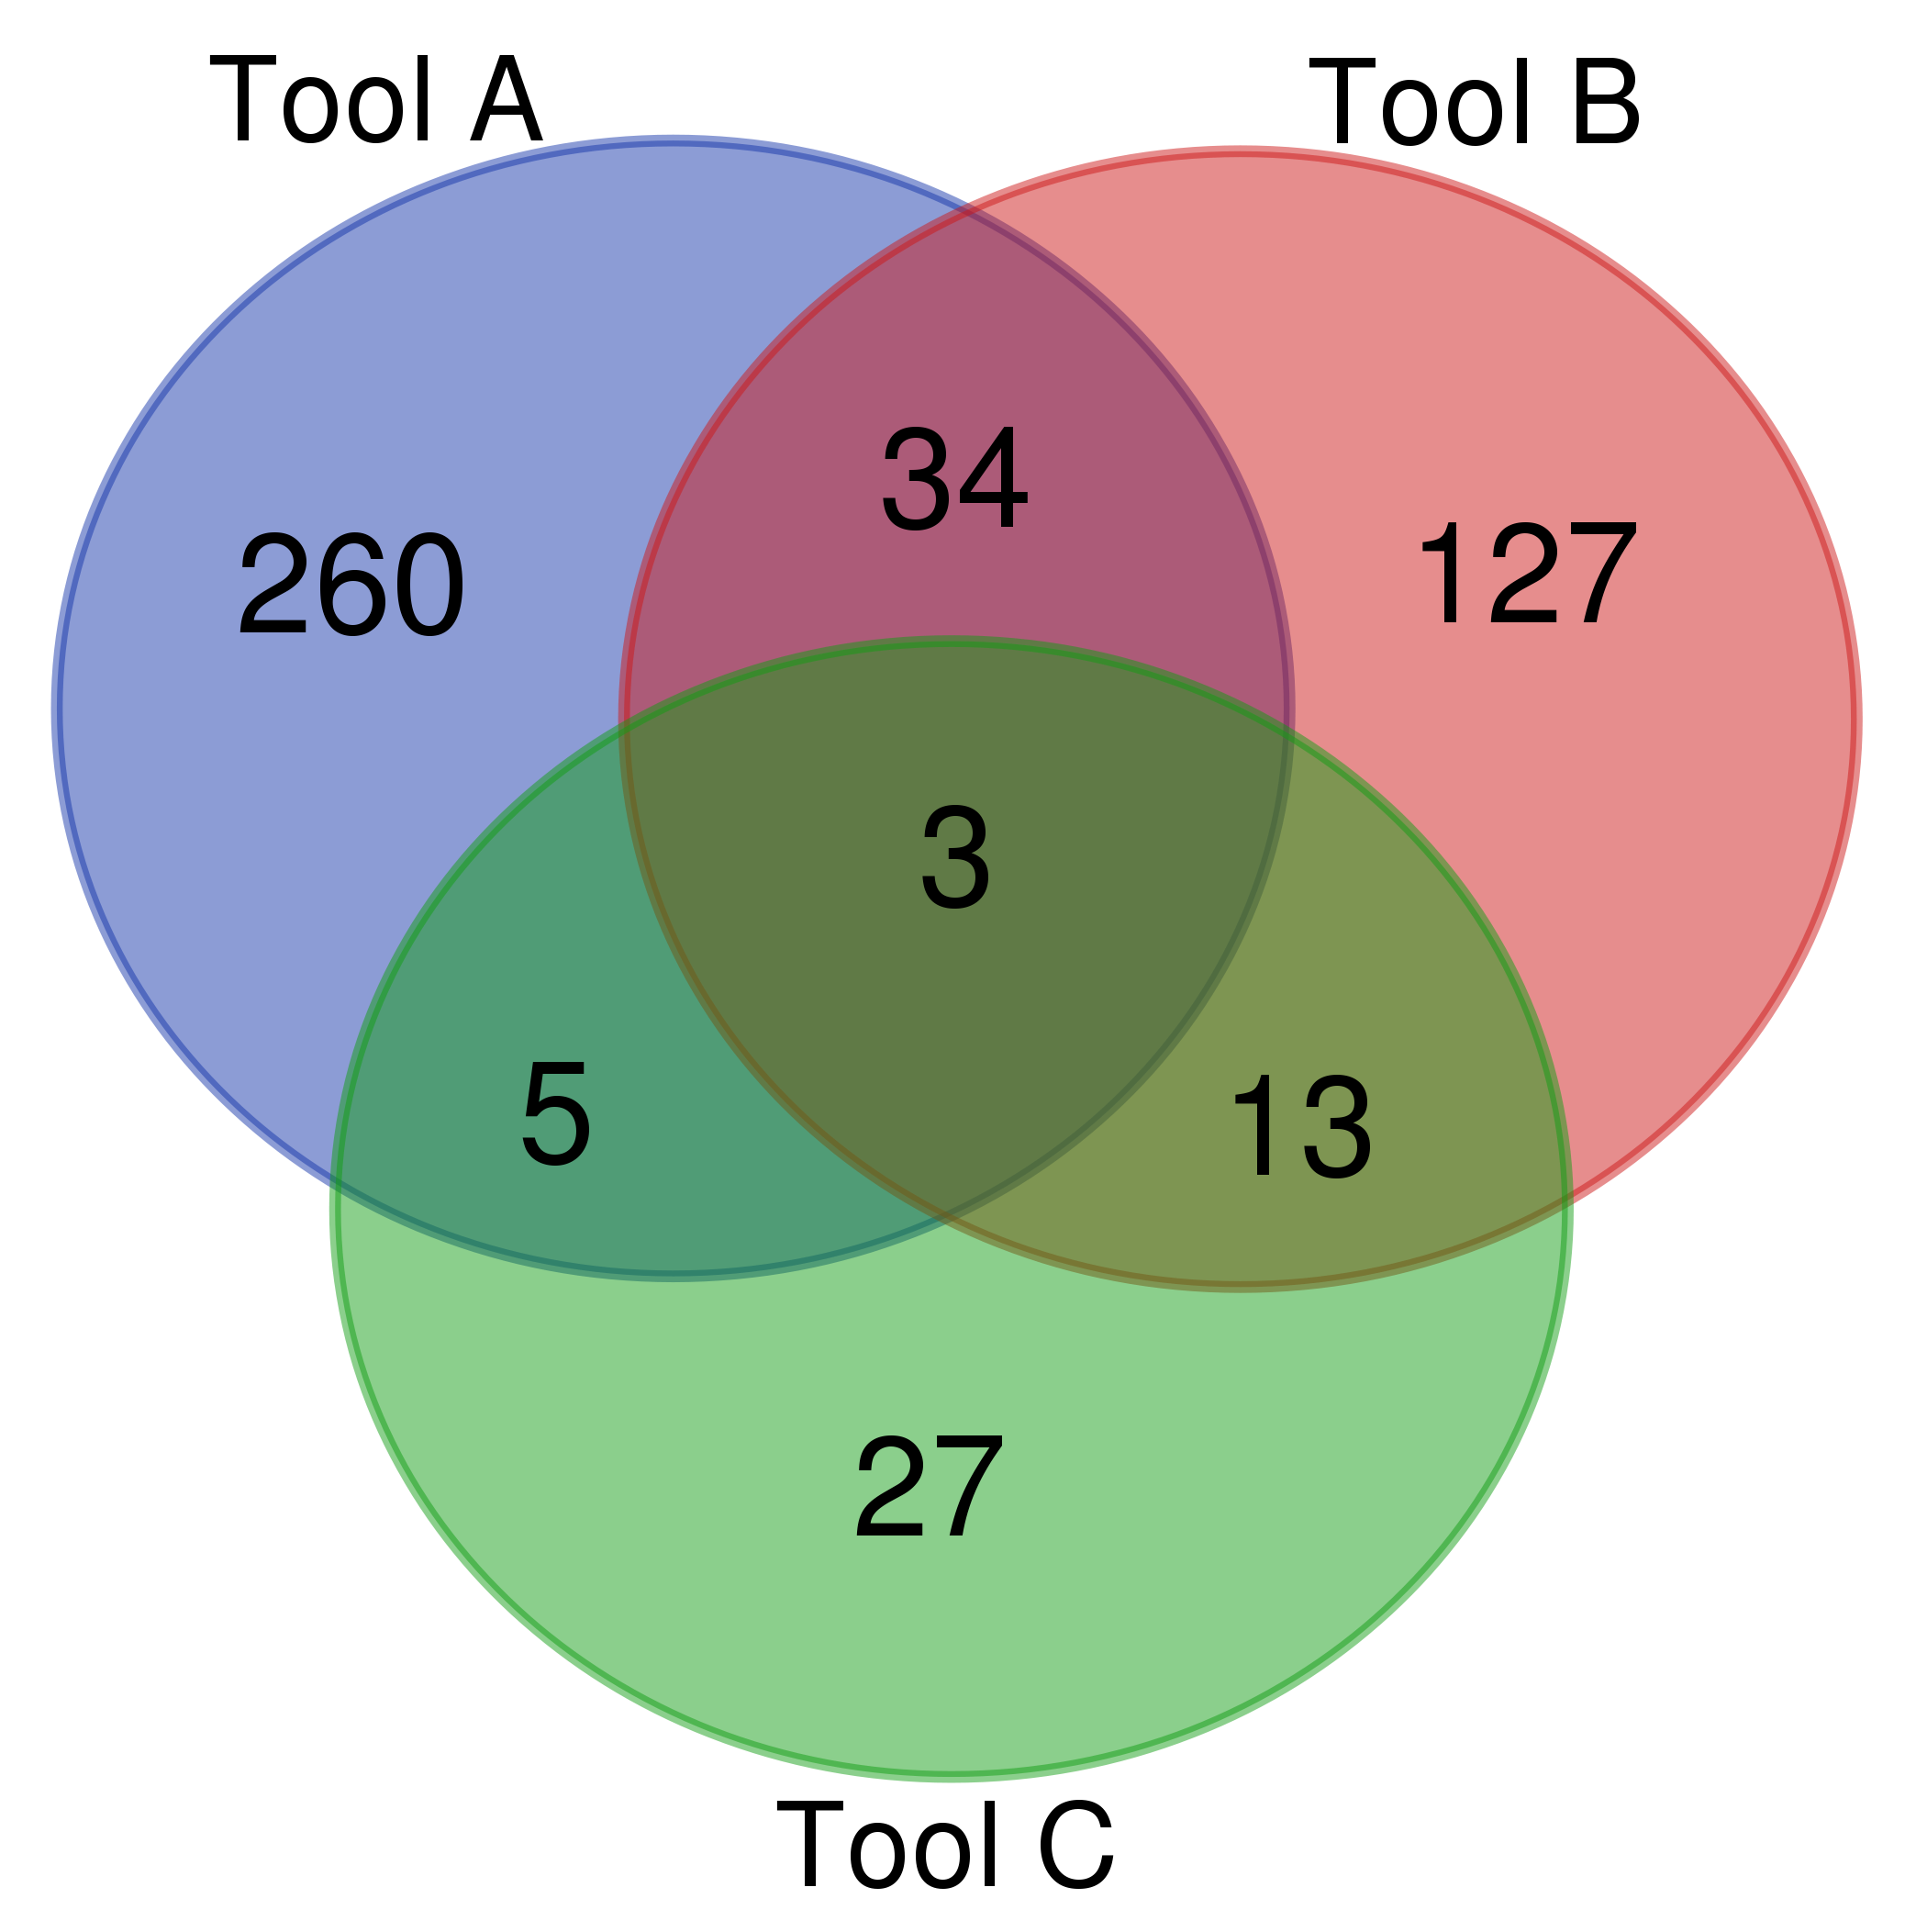
\includegraphics[width=0.30\columnwidth]{example.png}
  \caption{Mutants killed by three static analysis tools.}
  \label{fig:examplevenn}
\end{figure}

Finally, even when tools have similar quantitative results, examining individual mutants killed by one tool but not by another allows us to understand strengths and weaknesses of the tools, in a helpful context: the difference between the un-mutated code and mutated code will always be small and simple.  Moreover, simply looking at how much two tools agree on mutants can answer the question: given that I am using tool A, would adding tool B be likely be worthwhile?  Interested users, e.g. security analysts, can inspect the differences to get an idea of the particular cases when a tool might be most effective, but a more typical user can simply look at a Venn diagram of kills like that shown in Figure \ref{fig:examplevenn}.  Consider hypothetical tools A, B, and C.  A and B produce similar numbers of findings on the code in question, while tool C produces an order of magnitude more findings.  Tool A is likely the most important tool to make use of; it detected more mutants than any other tool, and more than twice as many mutants were killed by A alone than by B alone.  However, also running tool B is well justifed.  B does not do as well as A, but it is the only tool that detects a large number of mutants, and most mutants it detects are unique to it.  Finally, Tool C \emph{may} not be worth running, since its poor performance on mutants but high finding rate suggests it may be prone to missing bugs and to false positives.  It might be a good idea to just look at the 27 mutants detected by C alone:  \emph{if} they represent an important class of potential problems (perhaps C specialized in detecting potentially non-terminating loops), then C might be useful, but if the first few mutants inspected are false positives, then C is likely not useful.

\begin{figure}
{\scriptsize
\begin{code}
contract SimpleStorage \{
    uint storedData;

    function set(uint x) public \{
        storedData = x;
    \}

    function get() public view returns (uint) \{
        return storedData;
    \}
  \}
\end{code}
}
\caption{A simple example Solidity smart contract}
\label{fig:sol424intro}
\end{figure}

More concretely, consider the code in Figure \ref{fig:sol424intro} \cite{solintro}.  The Universal Mutator tool \cite{universalmutator,regexpMut}, which has been extensively tuned for Solidity's grammar (though not to target any particular vulnerabilities), and is the only smart contract mutation tool referenced in the Solidity documentation (\url{https://solidity.readthedocs.io/en/v0.5.12/resources.html}), produces seven valid, non-redundant (by Trivial Compiler Equivalence \cite{TCE}) mutants for it.  Both the public version of Slither \cite{slither} and SmartCheck \cite{smartcheck} (two popular smart contract static analysis tools) produce a small number (three and two, respectively) of low-severity, informational, warnings for this code.  Both tools also detect four of the seven mutants (here the number of warnings increases, and the additional warnings are clearly driven by the mutation change) .  However, only one of the mutants detected is common to both tools: both tools detect changing the {\tt return} statement in the {\tt get} function to a call to {\tt selfdestruct} the smart contract, deleting it.  Slither, but not SmartCheck, also detects replacing the assignment of {\tt storedData} in {\tt set} with either a {\tt selfdestruct} or {\tt revert}, or simply removing it altogether.  SmartCheck, on the other hand, detects removing the {\tt return} in {\tt get} or replacing it with a {\tt revert}, or removing the {\tt public} visibility modifier for {\tt get} \footnote{Slither's ``missing return'' detector is only available in the private version of slither, or through the {\tt crytic} service provided by Trail of Bits.}.  If we restrict our analysis to findings with a severity greater than informational, SmartCheck detects no mutants of the contract, while Slither still reports that some mutants \emph{allow an arbitrary caller to cause the contract to destroy itself}.  Given that both tools, ignoring informational results, detect no problems with the original code, and only Slither detects any problems with the mutants, we can say that Slither performs better for this contract.

Comparing mutant results also leads to the idea of \emph{improving} static analysis tools by examining mutants detected by another tool, and thus known to be in-principle detectable.  Improving tools by adding detectors is useful because, even if all tools had the same set of detectors, they would not all report the same bugs; different choices in intermediate language and tradeoffs made to avoid false positives may make the use of multiple tools with similar detectors essential for thorough analysis.  And if one tool simply has a superior engine, it is beneficial to users that the ``best'' tool incorporate \emph{all} detection rules.
However, as with efforts to improve test suites, manually searching through all mutants can be an onerous task, especially for large-scale evaluations.  We therefore introduce the idea of \emph{prioritizing} mutants to make it easier to inspect \emph{different} weaknesses in tools.

A general objection to our approach is that mutants may differ substantially from ``real'' faults, in some way.  This is certainly true, in a sense \cite{GopinathMutants}, but for static analysis purposes we believe it does not matter.   The real risk is that some mutation operators align with patterns a particular tool identifies, biasing the evaluation in favor of that tool.  Such faults may be dis-proportionately present in mutants vs. real code.  However, we consider this unlikely.  The vast majority of applied mutation operations for all of our experiments were highly generic, and do not plausibly represent a pattern in which some tool might specialize.  Code deletions, the most common kind of mutation by far, leave no ``trace'' for a tool to match against, but only an omission, so cannot be subject to this concern.  Changing arithmetic and comparison operators and numeric constants (incrementing, decrementing, or changing to 0 or 1) account for most of the non-statement-deletion mutants, and it is difficult to imagine how any tool could unfairly identify these.

%\subsection{Contributions}

This paper offers the following contributions:

\begin{itemize}[labelsep=3pt,leftmargin=12pt]
\item We propose a differential approach to comparing static analysis tools based on the insight that program mutants are easy-to-understand, likely-faulty, program changes.
\item We propose a definition of mutant killing for static analysis.
\item We introduce a simple scheme for prioritizing mutants that helps users understand and use the results of analysis.
\item We apply our method to an extensive, in-depth comparison of three Solidity smart contract analysis tools, and show how prioritization allowed us to easily identify (and build) three new detectors for the most effective of these tools.
\item We also provide results for popular Java and Python static analysis tools, further demonstrating our approach and showing strengths and weaknesses of these tools.
\end{itemize}

 While there are limitations to using differential mutation analysis to compare/improve static analysis tools, it scales to basing comparisons on many real software source files and very many ``faults,'' but still offers some of the advantages of having humans establish ground truth.

 \section{Differential Mutation Analysis}
 \label{sec:method}

The proposed approach is simple in outline:

\begin{enumerate}
\item Run each tool on the unmutated source code target(s), and determine the \emph{baseline}: the number of (non-informational/stylistic) findings produced.
\item Generate mutants of the source code and run each tool on each mutant.  Consider a mutant killed if the number of findings for the mutated code is greater than the number for the baseline, un-mutated code.
\item Compute, for each tool, the \emph{mutant ratio}:  the mutation score ($\frac{|\mathit{killed}|}{|\mathit{mutants}|}$) divided by (mean) baseline.  If it is zero, use a baseline equal to either one or the lowest non-zero baseline for any tool in the comparison set\footnote{This problem seldom arises in practice.}.
\item (Optional): Discard all mutants not killed by at least one tool and all mutants killed by all tools.  What remains allows \emph{differential} analysis.
Examine the remaining mutants in the difference in \emph{prioritized} order.
\end{enumerate}

The most important step here is the computation of the \emph{mutant ratio}, which tells us about the ability of a tool to produce findings \emph{for mutants}, relative to its tendency to produce findings in general.  If a tool has a tendency to produce large numbers of findings compared to other tools, and this is paired with a tendency to detect more mutants as well, then the tool will not be penalized for producing many findings.  Assuming that real faults are relatively rare in the original, un-mutated code, the best result and best (highest) mutant ratio will be for a tool that produces comparatively few findings for un-mutated code, but detects a larger portion of mutants than other tools; the worst result will be a tool that produces lots of findings, but detects few mutants.  We will actually see some examples of this worst case.

\subsection{Prioritizing Mutants}
\label{sec:prioritizing}

One goal of our approach is to make it easy for tool developers to examine cases where one tool kills a mutant and another fails to, in order to identify patterns for new detectors or analysis algorithm problems.  Dedicated developers may also simply want to scan all mutants their tool does not kill, for the same purpose, analogous to what Groce et al. have proposed for automated verification and testing \cite{groce2015verified,groce2018verified}.  Security analysts and other expert users who are not developers may also wish to do this, to better understand tool strengths and weaknesses.

Unfortunately the full list of unkilled mutants, or differentially
unkilled mutants, is likely to be both large and highly redundant.  In
our results below, only one of 9 tools we examined killed fewer than
1,000 mutants it alone detected.  Any cross-tool comparison is thus
likely to involve hundreds or thousands of mutants.

The problem of identifying unique ``faults'' (tool weaknesses) in this
situation is very similar to the \emph{fuzzer taming} problem in
software testing, as defined by Chen et al. \cite{PLDI13}: ``Given a
potentially large collection of test cases, each of which triggers a
bug, rank them in such a way that test cases triggering distinct bugs
are early in the list.'' \cite{PLDI13}.  Their solution was
to use Gonzalez' Furthest-Point-First \cite{Gonzalez} (FPF) algorithm
to \emph{rank} test cases so that users can examine very different
test cases as quickly as possible.  An
FPF ranking requires a distance metric $d$, and ranks items so that
dissimilar ones appear earlier.
The hypothesis of Chen et al. was that dissimilar tests, by a
well-chosen metric, will also fail due to different faults.  FPF is a
greedy algorithm that proceeds by repeatedly adding the item with the
\emph{maximum minimum distance to all previously ranked items}. Given an
initial seed item $r_0$, a set $S$ of items to rank, and a distance
metric $d$, FPF computes $r_i$ as
$s \in S: \forall s' \in S: min_{ j < i}(d(s,r_j)) \geq min_{j <
  i}(d(s',r_j))$.  The condition on $s$ is obviously true when
$s = s'$, or when $s' = r_j$ for some $j < i$; the other cases for
$s'$ force selection of \emph{some}
max-min-distance $s$.

In order to apply FPF ranking to examining mutants, we implemented a
simple, somewhat \emph{ad hoc} distance metric and FPF ranker.  Our metric $d$ is
the sum of a set of measurements.  First, it adds a similarity
ratio based on Levenshtein distance \cite{lev} for (1) the \emph{changes} (Levenshtein edits) from
the original source code elements to
the two mutants,  (2) the two original source code elements changed (in
general, lines), and (3) the actual output mutant code.  These are
weighted with multipliers of 5.0, 0.1, and 0.1, respectively; the type
of change (mutation operator, roughly) dominates this part of the
distance, because it best describes ``what the mutant did''; however,
because many mutants will have the same change (e.g., changing {\tt +}
to {\tt -}, the other ratios also often matter.
Our metric also incorporates a measure of the distance in the source
code between the locations of two mutants.  If the mutants are to
different files, this adds 0.5; it also adds 0.025
times the number of source lines separating the two mutants if they
are in the same file, but caps the amount added at
0.25.  

We do not claim this is an optimal, or even tuned, metric. Devising a better metric is left as future work, we only wish to show 
that even a hastily-devised and somewhat arbitrary metric provides 
considerable advantage over wading through an un-ordered list of 
mutants, and introduce the idea of using FPF for mutants, not just for tests: FPF is useful for failures in general, however discovered.

%; in the long
%run, it even may be completely replaced.  However, the metric we use
%provided useful results for a different problem, ranking mutants in an
%effort similar to that of Groce et
%al. \cite{groce2015verified,groce2018verified} to examine unkilled
%mutants for a smart contract library tested using the Echidna fuzzer \cite{echidna-code},
%and we simply adopted it for our differential mutation analysis.

\section{Experimental Results}

Our primary experimental results are a set of comparisons of tools using our method, for three languages: Solidity (the most popular language for smart contracts), Java, and Python.  We used the Universal Mutator tool for all experiments; for Solidity and Python, we believe the Universal Mutator is simply the best available tool.  For Java, PIT \cite{pitmut} is more popular, but does not produce source-level mutants, needed for PMD and for manual inspection of results.
We used our results to answer a set of research questions:

\begin{itemize}[labelsep=3pt,leftmargin=12pt]
\item {\bf RQ1:}  Does mutation analysis of static analysis tools produce actionable results?  That is, do raw mutation kills serve to distinguish tools from each other, or are all tools similar?
\item {\bf RQ2:}  Does our approach provide additional information beyond simply counting findings for the original, un-mutated analyzed code?  Do \emph{ratios} differ between static analysis tools?
\item {\bf RQ3:}  Do the rankings that raw kills and ratios establish agree with other sources of information about the effectiveness of the evaluated tools?  Can we independently confirm our results?
\item {\bf RQ4:}  Do tools detect more mutants in programs for which they produce no warnings, initially?
\item {\bf RQ5:}  Are mutants distinguishing tools usually flagged due to real faults, where the finding is related to the introduced fault; that is, are our results usually \emph{meaningful}?  
\item {\bf RQ6:}  Do individual mutants, prioritized for ease of examination, allow us to identify classes of faults that
 different tools are good at/bad at, and use this information to improve tools?  How does this compare to using mutants that have \emph{not} been prioritized?
  \end{itemize}

In particular, we consider {\bf RQ2} to be of critical importance; if the mutant ratios for tools differ, then this is clear evidence that our hypothesis that the tendency of mutants to be faults, and to expect that mutated code will, by a more precise and accurate tool, be flagged as problematic more often than non-mutated code, holds.  This expectation that (some subset of the) mutants can serve as proxies for real, detectable faults is the core concept of our approach.
{\bf RQ4} addresses a concern briefly mentioned in the introduction:  it is possible that warnings for the original code interfere with our definition of detection.  The ideal case for our approach is when a tool report no findings for un-mutated code, and either reports a finding (kills the mutant) or not (does not kill it) when the mutant is introduced.  Chekam et al. showed that the ``clean program assumption'' for testing, the idea that coverage will be similar for faulty and fixed versions of a program, is a threat to the validity of investigations of the relationship between coverage and fault detection \cite{CleanProgram}, and we want to establish that this is unlikely to be the case for our approach.  Our answer to {\bf RQ5} is somewhat inherently qualitative and incomplete; we cannot analyze all mutants on which results are based manually, and understanding the mutants and tool warnings completely would require deep understanding of all the software systems investigated.  However, in many cases, the impact of a mutant is clear, and the reason for warnings is obvious.  This was often enough the case that, as we discuss below, we are confident mutants that distinguish tools are meaningful (missed) opportunities for static analysis tools.
For {\bf RQ6}  we have only preliminary answers, for the smart contract tools.  

\subsection{Solidity Smart Contract Tools}

\subsubsection{Smart Contracts and Smart Contract Static Analysis}

Smart contracts are autonomous code instruments, usually operating on a blockchain, that often have critical responsibilities such as facilitating and verifying (large) financial services transactions, tracking high-value physical goods or intellectual property, or even controlling ``decentralized organizations'' with multifarious aspects.  Security and correctness are thus critical in the smart contract domain, and static analysis is a key way to ensure allocation of high-value resources is not compromised.  The most popular smart contract platform, by far, is the Ethereum blockchain, and the Solidity smart contract language \cite{buterin2013whitepaper,wood2014yellow}; the Ethereum cryptocurrency has a market capitalization as we write of over \$15 billion dollars, largely fueled by interest in the smart contract functionality.  Ethereum contracts have been the targets of widely publicized attacks, with large financial consequences  \cite{spank,DAO}.   A recent paper examining results from 23 professional security audits of Solidity contracts argues that effective static analysis is a major key to avoiding such disasters in the future \cite{FC20}.

\subsubsection{Static Analysis Tools Compared}

We analyzed three well-known tools for static analysis of Solidity smart contracts: Slither \cite{slither}, SmartCheck \cite{smartcheck}, and Securify \cite{Securify}.  Slither, based on an SSA-based intermediate language (SlithIR \cite{slither}) is an open-source tool from Trail of Bits.  SmartCheck, developed by SmartDec, translates Solidity source directly to an XML-based representation, then uses \emph{XPath} patterns to define problems.  Securify, from SRI Systems Lab at ETH Zurich, works at the bytecode level, first parsing and decompiling contracts, then translating to \emph{semantic facts} in order to look for predefined problems.

\subsubsection{Smart Contract Selection}

We could have used a set of high-transaction contracts, or known-important contracts to validate our approach.  However, we knew that one of our goals in the Solidity experiments was to actually improve a mutation analysis tool, and the developers of the static analysis tools use exactly such benchmarks to validate their tools.  Basing our improvements on mutants of the contracts used for evaluation of proposed detectors would introduce a serious bias in our favor: we would be more likely to produce detectors that would have true positives and few false positives on the benchmark contracts.  We therefore instead selected 100 random contracts for which EtherScan (\url{https://etherscan.io/}) has source code, and used this (quite arbitrary) set of contracts from the actual blockchain to compare tools and identify opportunities for improvement.  The collected contracts had a total of 15,980 non-comment source lines, as measured by {\tt cloc}, with a mean size of 159.8 LOC and a median size of 108 LOC.  The largest single contract had 1,127 lines of code.  The Universal Mutator generated 46,769 valid mutants for these 100 contracts.

\subsubsection{Analysis Results}

\begin{figure}
  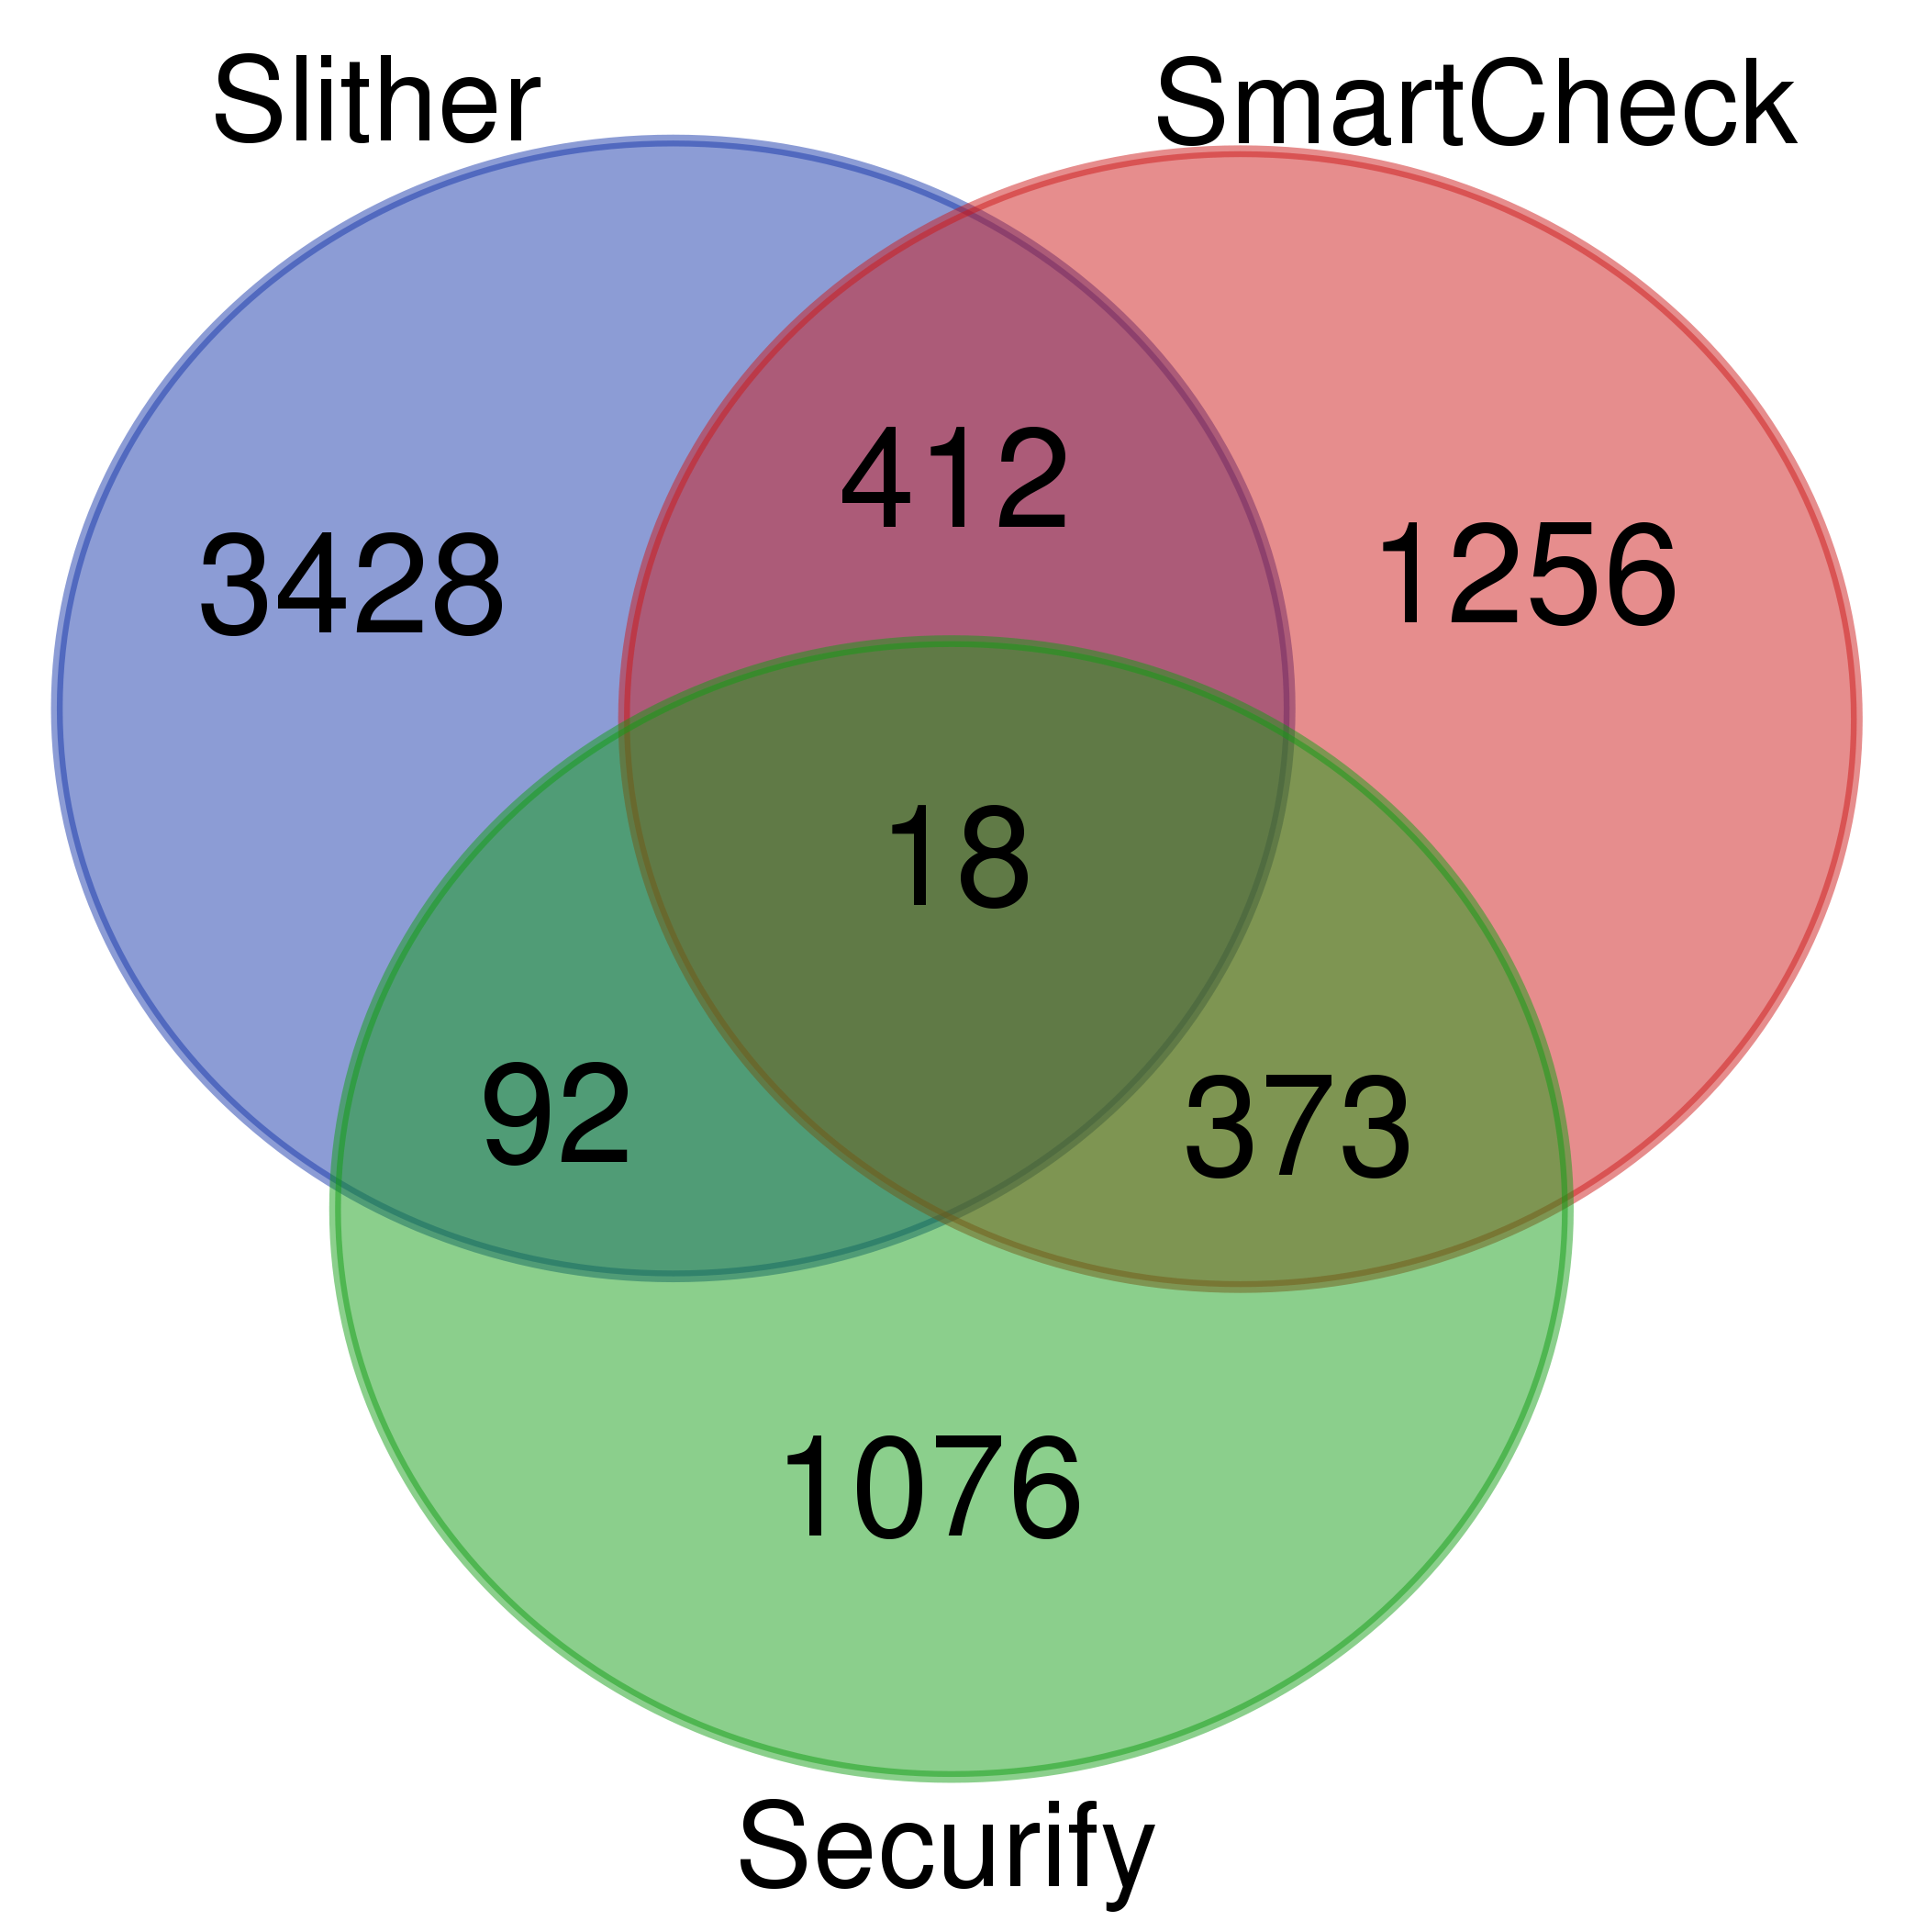
\includegraphics[width=0.35\columnwidth]{solidity.png}
  \caption{Mutants killed by Solidity static analysis tools.}
  \label{fig:solidityvenn}
\end{figure}

\begin{table}
  \begin{tabular}{l|r|r|r|r|r}
    & \multicolumn{2}{|c|}{Findings} & \multicolumn{2}{|c|}{Mutation Score}  & Mutant \\
    Tool & Mean & Median & Mean & Median & Ratio\\
    \hline
    \hline
    Slither & 2.37 & 1.0 & 0.09 & 0.09 & 0.038 \\
    Clean (39) & - & - & 0.11 & 0.11 & -\\
    \hline
    SmartCheck & 1.89 & 1.0 & 0.05 & 0.05 & 0.026 \\
    Clean (27) & - & - & 0.03 & 0.01 & - \\
    \hline
    Securify & 24.65 & 17.0 & 0.03 & 0.02 &  0.001 \\
    Clean (5) & - & - & 0.00 & 0.00 & - \\
    \hline
    
  \end{tabular}
  \caption{Solidity tool results over all contracts.}
  \label{tab:scoresolidity}
\end{table}


Figure \ref{fig:solidityvenn} shows the mutants killed by the Solidity analysis tools.  Table \ref{tab:scoresolidity} provides numeric details of the results, including the \emph{ratio} for each tool, adjusting its mutation scores by its' general tendency to produce findings.  The second row for each tool shows the number of contracts for which it reported no findings, and the mutation scores over those contracts, only. A user examining these results would suspect that Slither and SmartCheck are both useful tools, and should likely both be applied in a high-risk security-sensitive context like smart contract development.  A user might also suspect that the large number of findings produced, and smaller number of mutants killed, for Securify, means that whether to apply Securify is a more difficult decision.  On the one hand, Securify does detect nearly as many mutants it alone can identify as SmartCheck.  The large number of findings, and very bad mutant ratio, however, lead us to suspect that many of these ``detected'' mutants are false positives (or, at least, that the problem is not the one Securify identifies).  Extracting the signal from Securify's noise will be difficult.  We also note that while running Slither and SmartCheck on all 46,769 valid mutants was relatively quick (it took about 6 days sequential compute time for Slither and 3 days for SmartCheck, i.e., about 5-15 seconds per mutant for both tools), Securify often required many hours to analyze a mutant, and frequently required a few days to analyze a mutant; the full analysis required over three months of compute time.

For our research questions, {\bf RQ1} is clearly answered in the affirmative.  Figure \ref{fig:solidityvenn} shows that the tools address quite different problems, with all tools reporting far more uniquely detected mutants than mutants in common with other tools.  There are only 18 mutants detected by all tools, all of them involving replacement of {\tt msg.sender} (the caller of a smart contract, which may be another smart contract) with {\tt tx.origin} (the original initiator of a sequence of blockchain calls, a ``human'' account).  Use of {\tt tx.origin} is often (though not always) a bad idea, and can lead to incorrect behavior, so it is not surprising tools all recognize some misuses of it.

{\bf RQ2} is also answered in the affirmative.  Counting findings for un-mutated code might suggest that Securify is the best tool, by a wide margin, but in the context of its near-zero mutant ratio, we must suspect that many of the warnings are false positives.  Slither has the best mutant ratio, but the margin between it and SmartCheck confirms that both tools likely provide value.

For {\bf RQ3}, there are only a few tool comparisons in the literature; this is probably due to the fast-moving nature of the blockchain analysis world; the oldest of these tools' publication dates is 2018.  The most extensive is that of Durieux et al. \cite{durieux2019empirical}, though it unfortunately was unable to provide anything other than an implicit look at false positives, somewhat limiting its practicality.  Slither detected 17\% of known vulnerabilities in their analysis, vs. 11\% for SmartCheck and 9\% for Securify. Slither and SmartCheck were also among the four (out of 9) tools that detected vulnerabilities in the most categories; Securify was not.  The overall recommendation of Durieux et al. was to use a combination of Slither and Mythril \cite{mythril-code} for contract analysis.  Parizi et al. \cite{Parizi} also offer a ranking of tools, and determined that SmartCheck was the most effective, and far more so than Securify; unfortunately, they did not include Slither in their set of evaluated tools.

The Slither paper \cite{slither} also provides an evaluation of all three tools.  Their findings counts differ from ours because of different choices (we threw out merely informational results), but these are unrelated to mutation analysis, in any case.  The evaluation only considered reentrancy faults \cite{SurveyAttacks,FC20} (which are sometimes, but only rarely, introduced by mutants).  For reentrancy, Slither performed best on two real-world large contracts, finding subtle bugs in both, SmartCheck detected the problem in one of the two, and Securify detected neither.  For a set of 1,000 contracts, SmartCheck had a high false positive rate (over 70\%) but detected more actual reentrancies (209) than Slither (99) or Securify (6).  On the other hand, Slither's low false positive rate of 11\%  makes its results possibly more useful in practice.

For {\bf RQ4}, on the changes seen when restricting analysis to clean contracts, Slither did slightly better at detecting mutants when the original contract was clean for Slither, and the other two tools did somewhat worse on contracts for which they reported no findings.  For the three contracts clean for all tools, Slither performed almost exactly as it did over contracts in general, and the other tools performed worse, by about the same margin as they did for their own clean contracts.  For our approach, we only need a weak version of the ``clean program assumption'':  the threat is that kills may be under-reported for non-clean programs, due to interference with findings for the original code.  It is not a problem if mutation scores are \emph{worse} for programs where a tool reports no findings for the un-mutated code.  We therefore, for smart contracts, find no threat to our approach arising from the presence of findings on un-mutated code.  We speculate that ``clean'' results for some tools result from contracts where the tool has trouble with the contract code, but does not actually crash; Slither may do better on clean code because it has fewer such failures, and clean contracts are probably generally simpler and easier to analyze.

Because examining all mutants manually is infeasible,  for {\bf RQ5} we focused primarily on examining mutants in the \emph{difference}: mutants detected by at least one tool, but not detected by all tools, the only ones that actually influence the comparison of tools.  The vast majority of the mutants in this set were meaningful semantic changes a static analysis tool could be expected to detect, and the findings produced by tools were relevant to the nature of the fault.  We do not believe that all mutants represent definite faults; some are harmless but unusual code changes.  A large number of the instances where use of {\tt tx.origin} in place of {\tt msg.sender} was flagged seem to us to be strange, but not necessarily incorrect, code.  On the other hand, at the risk of false positives, it is not unreasonable for tools to report such strange code.   Our estimate is that, ignoring {\tt tx.origin} cases, \emph{at least 70\% of the mutants detected by one, but not all, tools, represent realistic bugs}, and failure to detect is roughly equally due to missing detectors and imprecise analysis.

Because our random contracts' quality might be low, we also checked our results on 30 contracts from the Solidity documentation, the \emph{Mastering Ethereum} book \cite{masteringEth}, and a handful of selected, recent, higher quality blockchain contracts.  Slither had a mean mutation score of 0.11, vs. 0.04 for SmartCheck and 0.01 for Securify.  Associated mutant ratios were 0.38, 0.08, and 0.007.  Mutant kill overlap was also similar; in fact, Figure \ref{fig:examplevenn} shows the results: Slither is A, SmartCheck is B, and Securify is C.

\subsubsection{Improving Slither {\bf (RQ6)}}

Based on the differential mutation analysis, we identified three low-hanging fruit to improve the performance of Slither.  We chose Slither in part because it seems to have a better underlying intermediate language and analysis engine, and thus is likely to produce better results for the same rule than the other tools.  The process was simple.  First, we produced a list of all mutants killed by either SmartCheck or Securify, but not killed by Slither.  We then applied the prioritization method based on the FPF algorithm and the distance metric described in Section \ref{sec:prioritizing}, and examined the mutants in rank order.  Many of the mutants were difficult to identify as true or false positives, absent context.  Some opportunities for enhancement were clear, but seemed likely to require considerable effort to implement without producing a large number of false positives.  For example, Securify often detected when an ERC20 token contract's guard preventing making the special 0x0 address the owner of a contract was removed, and issued the error {\tt Violation for MissingInputValidation}. Detecting such missing guards is probably useful, but doing so without producing false positives is non-trivial.  We wanted to show that mutants could identify \emph{useful} but \emph{easy to implement} missing detectors.  Examining only a few mutants, we identified three:

\begin{figure}
  {\scriptsize
      {\bf Mutant showing Boolean constant misuse.}

    
\noindent \begin{code}
 0x598ab825d607ace3b00d8714c0a141c7ae2e6822\_Vault.mutant.275.sol:
 if (!p.recipient.send(p.amount)) \{  // Make the payment
 ==>          if (true) \{  // Make the payment
 if (true) \{  // Make the payment
      \end{code}

      }

      {\scriptsize
              {\bf Mutant showing Type-based tautologies.}
\begin{code}
 0x968815CD73647C3af02a740a2438D6f8219e7534\_TTPresale.mutant.311.sol:
 require(nextDiscountTTMTokenId6 >= 361 \&\& nextDiscountTTMTokenId6 <= 391);
 ==>  ...361...==>...0...
 require(nextDiscountTTMTokenId6 >= 0 \&\& nextDiscountTTMTokenId6 <= 391);
      \end{code}
      }


      {\scriptsize
      {\bf Mutant showing Loss of precision.}        
\begin{code}
 0x534ccee849a688581d1b0c65e7ff317ed10c5ed3\_NametagToken.mutant.480.sol:
 byte char = byte(bytes32(uint(x) * 2 ** (8 * j)));
 ==>  ...*...==>.../...
 byte char = byte(bytes32(uint(x) * 2 ** (8 / j)));
      \end{code}

}
        \caption{Examples of mutants leading to new detectors.}
       \label{fig:newdetect}
    \end{figure}

\begin{enumerate}
\item {\bf Boolean constant misuse:}  This detector flags code like {\tt if (true)} or {\tt g(b || true)} (where {\tt g} is a function that takes a Boolean input).  Constant-valued conditionals tend to indicate debugging efforts that have persisted into production code, or other faults; there are almost no circumstances where a conditional should not vary with state or input.  This detector is actually split into two detectors, one for this serious issue, and an informational/stylistic detector that notes that code such as {\tt if (x == true)}, while semantically harmless, is difficult to read.  This problem was easily identified from cases such as the mutant in Figure \ref{fig:newdetect}, killed by SmartCheck but not Slither:

\item {\bf Type-based tautologies:}  A type-based tautology is again a case where a Boolean expression has a constant value, but this is not due to misuse of a Boolean constant, but is instead due to the \emph{types} in a comparison.  For example, if {\tt x} is an unsigned integer type, the comparison {\tt x >= 0} is always true and {\tt x < 0} is always false.  This detector is a generalization of the SmartCheck detector \url{https://github.com/smartdec/smartcheck/blob/master/rule\_descriptions/SOLIDITY\_UINT\_CANT\_BE\_NEGATIVE/}, modified to actually compute the ranges of types and identify more general instances of tautological comparisons, e.g. {\tt y < 512} where {\tt y}'s type is {\tt int8}.  Again, the problem was easily identified by mutants killed by SmartCheck but not Slither.

\item {\bf Loss of precision:}  Solidity only supports integer types.  This means that performing division before multiplication can introduce rounding that is not present when the multiplication is performed first.  This is a fairly important problem, given the frequency with which Solidity code performs financial calculations where maximum precision is desired.  SmartCheck provides a detector for such precision losses \url{https://github.com/smartdec/smartcheck/blob/master/rule\_descriptions/SOLIDITY\_DIV\_MUL/}.
\end{enumerate}      

All three of these detectors were submitted as PRs, vetted over an internal benchmark set of contracts used by the Slither developers to evaluate new detectors, and accepted for release in the public version of Slither.  All three detectors produce some true positives (actual problems, though not always exploitable) in benchmark contracts, have acceptably low false positive rates, and were deemed valuable enough to include as non-informational (medium severity) detectors.  The first mutants in prioritized rank exhibiting the issues, shown above, were the 2nd, 9th, and 12th non-statement-deletion mutants ranked for SmartCheck, out of over 800 such mutants.  Using our prioritization, it was possible to identify these issues by examining fewer than 20 unkilled mutants.  Without prioritization, on average a developer would have to look at more than 200, 80, and 400 mutants, respectively, to find instances of these problems.  Interestingly, the very fact that these instances are ``needles in a haystack'' among the mutants not killed by Slither means that the results in Figure \ref{fig:solidityvenn} and Table \ref{tab:scoresolidity} are almost unaltered by our improvements to Slither: our analysis is fairly robust to modest tool improvements, unless added detectors account for a large number of mutants not detected by the tool.  Adding such detectors will also only improve mutation ratio if they do not add many false positives.  Substantial changes in results therefore require adding very effective (for mutants) detectors that seldom trigger for correct code (or at least trigger much less than for mutants).  ``Cheating'' with respect to a mutation benchmark is thus, we hope, difficult without actual major tool improvements.

There were 92 separately ranked statement deletion mutants also.  These, however, could all be ignored, as they were almost entirely duplicates related to the missing-return statement detector.  If this detector were not already present as a private Slither detector, it would also be a good candidate for addition to the tool.  Our three submitted detectors were not present as private detectors, and only one (the type-based tautology detector) had even been identified, via a GitHub issue, as a potential improvement (and only in the private version of Slither).  Combining statement deletion mutants with other mutants only moved the mutants we used down to 3rd, 11th, and 14th positions.  By default we rank statement deletions separately, since such mutants are usually easier to understand and either note as important or dismiss, and in testing (but not static analysis) they are likely to be the most critical faults not detected.

Examining the first 100 mutants in the unprioritized lists for SmartCheck and Securify, ordered by contract ID and mutant number (roughly source line mutated) we were unable to identify \emph{any} obviously interesting mutants, suggesting that it is indeed hard to use mutation analysis results without prioritization. A large majority of the mutants we inspected involved either the missing
{\tt return} problem noted in the introduction, or replacing {\tt msg.sender} with {\tt tx.origin}; Slither has a detector for misuses of {\tt tx.origin}.  SmartCheck and Securify tend to identify most (though not all) uses of {\tt tx.origin} as incorrect, while Slither has a more selective rule, intended to reduce false positives.
It is hard to scale our efforts here to a larger experiment, since writing and submitting changes to static analysis tools is always going to be a fairly onerous task, but we believe that our successful addition of new detectors, and the ease of identifying good candidate detectors using mutant prioritization supports a limited affirmative answer to {\bf RQ6}.

\subsection{Java Tools}

\subsubsection{Static Analysis Tools Compared}

For Java, we again compared three tools.  SpotBugs (\url{https://spotbugs.github.io/}) is the ``spiritual successor'' of FindBugs \cite{FindBugs,CompareJavaTools}.  PMD (\url{https://pmd.github.io/}) \cite{CompareJavaTools} is an extensible cross-language static code analyzer.  FaceBook's Infer (\url{https://fbinfer.com/}) \cite{Infer} focuses on diff-related detection of serious errors (concurrency, memory safety, and information flow).

\subsubsection{Project Selection}

For Java and Python, we did not have to worry about invalidating tool improvements by basing our results on benchmark code.  We therefore aimed to use realistic, important source code.  We selected top GitHub projects (defined by number of stars) for each language, and removed projects with fewer than 5 developers or less than six months of commit history (as well as projects that did not build).  For Java, we analyzed the top 15 projects satisfying our criteria, with a maximum of 623,355 LOC and a minimum of 3,957 LOC, and a total size of 1.8 million LOC.  Because the Universal Mutator does not ``know'' Java syntax, and Java is very verbose, the Java compiler rejected a large number of the generated mutants (e.g., deleting declarations).  We still, due to the huge size of the source files and thus number of mutants (and time to compile full projects), restricted our analysis to files where Universal Mutator's implementation of TCE \cite{TCE} for Java was useful, i.e. files that could be compiled and the bytecode compared without processing the full project, leaving us with just over 70,000 mutants, ranging from 136 to 10,016 per project.

\subsubsection{Analysis Results}


\begin{figure}
  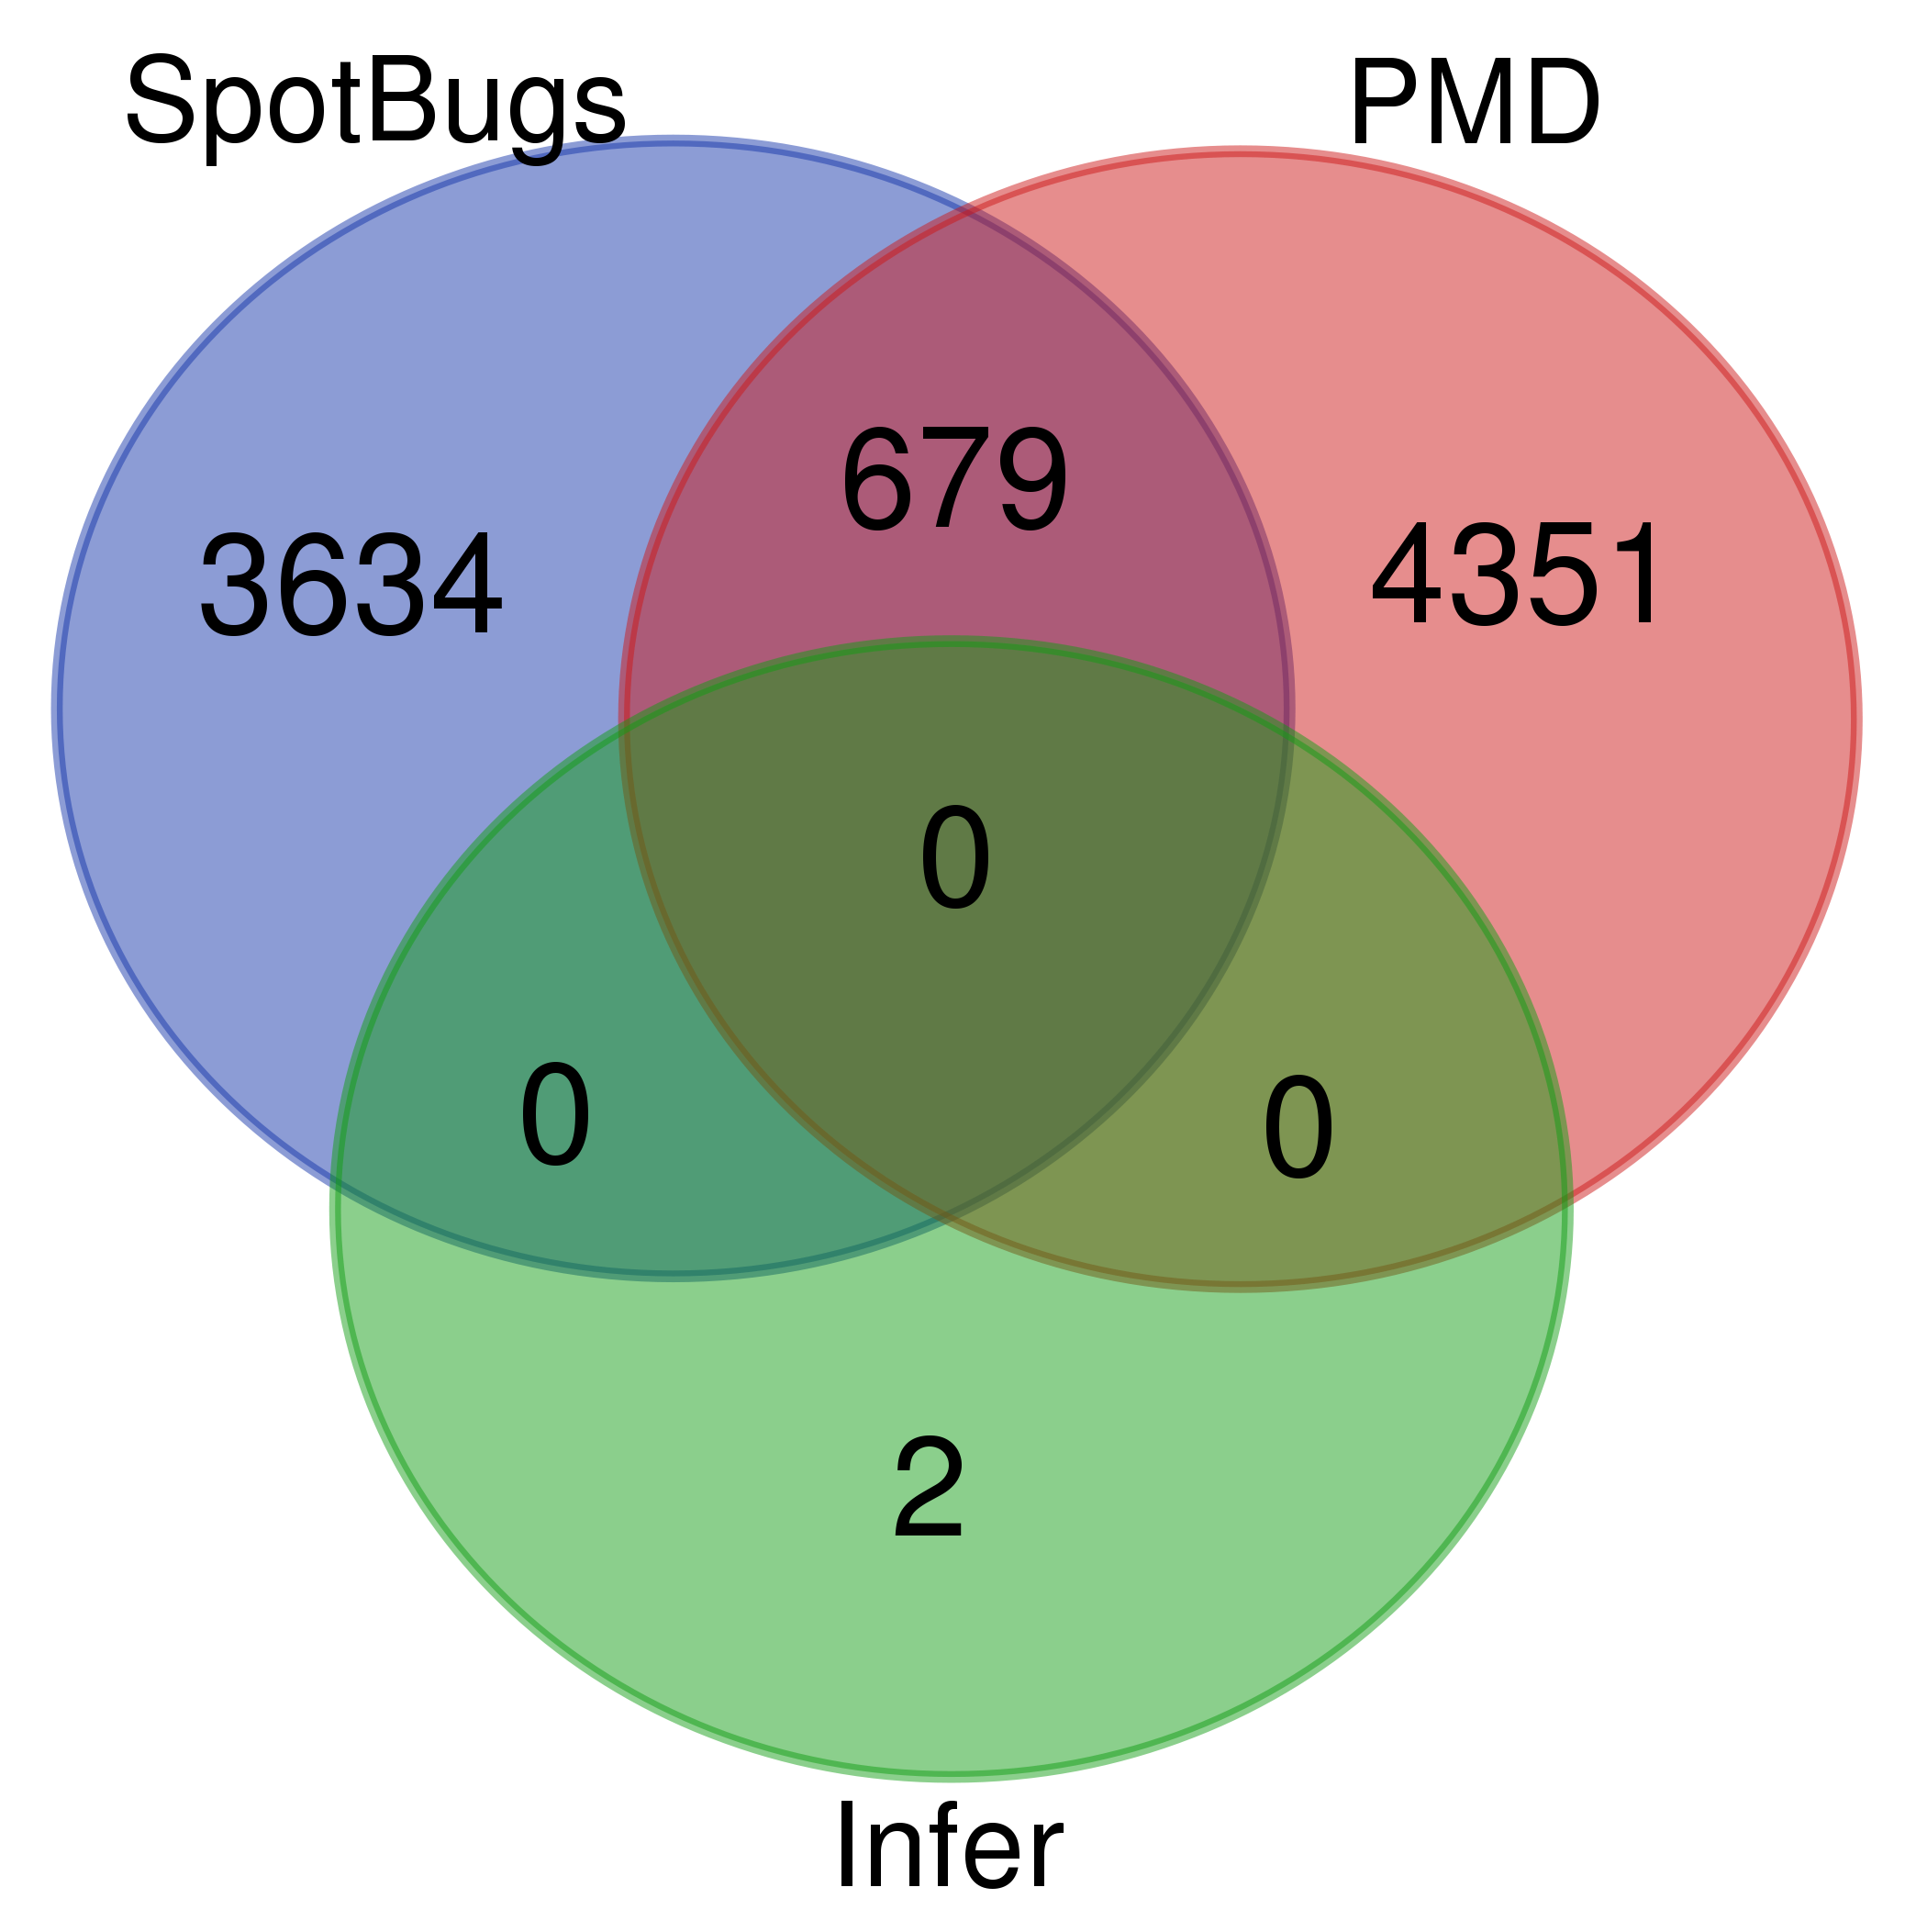
\includegraphics[width=0.35\columnwidth]{java.png}
  \caption{Mutants killed by Java static analysis tools.}
  \label{fig:javavenn}
\end{figure}

\begin{table}
  \begin{tabular}{l|r|r|r|r|r}
    & \multicolumn{2}{|c|}{Findings} & \multicolumn{2}{|c|}{Mutation Score}  & Mutant \\
    Tool & Mean & Median & Mean & Median & Ratio\\
    \hline
    \hline
    SpotBugs & 28.93 & 14.00 & 0.07 & 0.07 & 0.002 \\
    Clean (3) & - & - & 0.05 & 0.06 - \\
    \hline
    PMD & 53.73 & 32.00 & 0.07 & 0.07 & 0.001 \\
    Clean (0) & - & - & - & - & - \\
    \hline
    Infer & 11.60 & 3.00 & 0.00 & 0.00 &  0.000 \\
    Clean (6) & - & - & 0.00 & 0.00 \\
    \hline
  \end{tabular}
  \caption{Java tool results over all projects.}
  \label{tab:scorejava}
\end{table}



Figure \ref{fig:javavenn} shows the mutants killed by the Java analysis tools, and Table \ref{tab:scorejava} provides numeric results for projects and clean projects, respectively.

In terms of {\bf RQ1}, the raw kills results suggest there is considereable value in running both SpotBugs and PMD.  Both produce a large number of unique detections, though PMD produces about 20\% more than SpotBugs.
Infer on the other hand, is only able to detect two mutants, but these are unique.  Unfortunately, these mutants only served to indicate that we were actually running Infer in such a way that it \emph{could} detect problems:  both were concurrency warnings, but the code change in both cases was simply removing a (semantically inoperative) {\tt \@Override} annotation.  It may be that the diff sizes in our code were simply too small for Infer's approach.
{\bf RQ2} is also answered in the affirmative.  While the raw kills for SpotBugs are not as good as for PMD, it produced fewer findings, giving it a mutant ratio approximately twice that of PMD.

We note that SpotBugs crashed for many more Java programs than PMD and Infer (neither crashed for any original file in our experiments).  SpotBugs ``failed to detect'' 23,000 of the mutants because it did not process the un-mutated file for 383 files, over 12 of the 15 projects---just over 23\% of the 1,664 total files.  Removing files for which SpotBugs failed, however, did not dramatically change results; SpotBugs' mean mutation score rose to 0.09, and mutant ratio rose to 0.003, but PMD's mean score rose to 0.10, and mutant ratio to 0.002.

\begin{figure}
  {\scriptsize
    % \begin{itemize}
    \raggedright    
  \url{https://stackoverflow.com/questions/4297014/what-are-the-differences-between-pmd-and-findbugs} \\
  \url{https://www.sw-engineering-candies.com/blog-1/comparison-of-findbugs-pmd-and-checkstyle} \\
  \url{https://www.reddit.com/r/java/comments/3i7w6n/checkstyle_vs_pmd_vs_findbugs_for_dummies_why/} \\
  %\end{itemize}
  }
\caption{Discussions of Java static analysis tools.}
\label{fig:blog}
\end{figure}

For {\bf RQ3}, to our knowledge there is no academic comparison of all three tools; one study dates from 2004 \cite{CompareJavaTools}, used FindBugs, not SpotBugs, and reached no strong conclusions with respect to FindBugs vs. PMD; a more recent study found that SpotBugs outperformed Infer for Defects4J \cite{just2014defects4j} bugs \cite{AllBugs}, but did not compare to PMD.  However, the user postings listed in Figure \ref{fig:blog}, plus personal communications with security analysts who use these tools \cite{personalJava} supported some basic conclusions.  SpotBugs is perhaps the best tool for finding bugs; PMD focuses more on stylistic issues and has a weaker semantic model.  Running both is definitely recommended, as neither is extremely effective.  Infer is closer to a model checker focusing on resource leaks than a truly general-purpose tool, arguably.  In fact, we suspect Infer would perform much better if we crafted complex mutation operators targeting some important subtle Java bugs; it is still fair to say that Infer is probably not a good \emph{general-purpose} static analysis tool for Java.  Note that we did not use Infer's experimental, non-standard, detectors, however.

For {\bf RQ4} there were very few clean projects, but the mutation scores for Infer were unchanged, and for SpotBugs they were worse.  We see no evidence that non-clean code is a source of degradation in mutation detection.

For Java, again, the large majority of mutants we inspected for {\bf RQ5}, where at least one tool detected the mutant and at least one tool did not detect it were definitely meaningful.  In particular, for Java, the large majority of mutants involved either deleted method calls or changes to conditionals (e.g., {\tt == null} to {\tt != null}) that would clearly introduce potential null pointer exceptions (NPEs), and such a possible NPE was the produced finding.  While the differences between Solidity tools were often due to different detectors, the Java differences seemed mostly rooted in analysis engine methods; all tools aim to warn about potential NPEs.  Because the number of mutants we could examine and understand was smaller, we are less confident in making a probabilistic estimate than with Solidity, but it was clear the basis of the comparison was primarily realistic faults, which some tools detected and others did not.

\subsection{Python Tools}

\subsubsection{Static Analysis Tools Compared}

We compared three widely used and well-known Python tools:  Pylint \url{https://www.pylint.org/} (probably the most widely used of Python bug finding tools), pyflakes \url{https://pypi.org/project/pyflakes/}, designed to be faster, lighter-weight, and more focused on bugs (without configuration) than Pylint, and PyChecker \url{http://pychecker.sourceforge.net/}, an older, but still used (e.g., we found numerous {\tt .travis.yml} files installing and running PyChecker), tool.

\subsubsection{Project Selection}

For Python, we analyzed the top 25 GitHub projects by our criteria (see above), due to the smaller size of Python projects.  These ranged in size from 3,377 LOC to 34,671 LOC, with a total size of just under 100 KLOC.  For Python, we were able to produce 167,511 valid mutants to analyze.

\subsubsection{Analysis Results}


\begin{figure}
  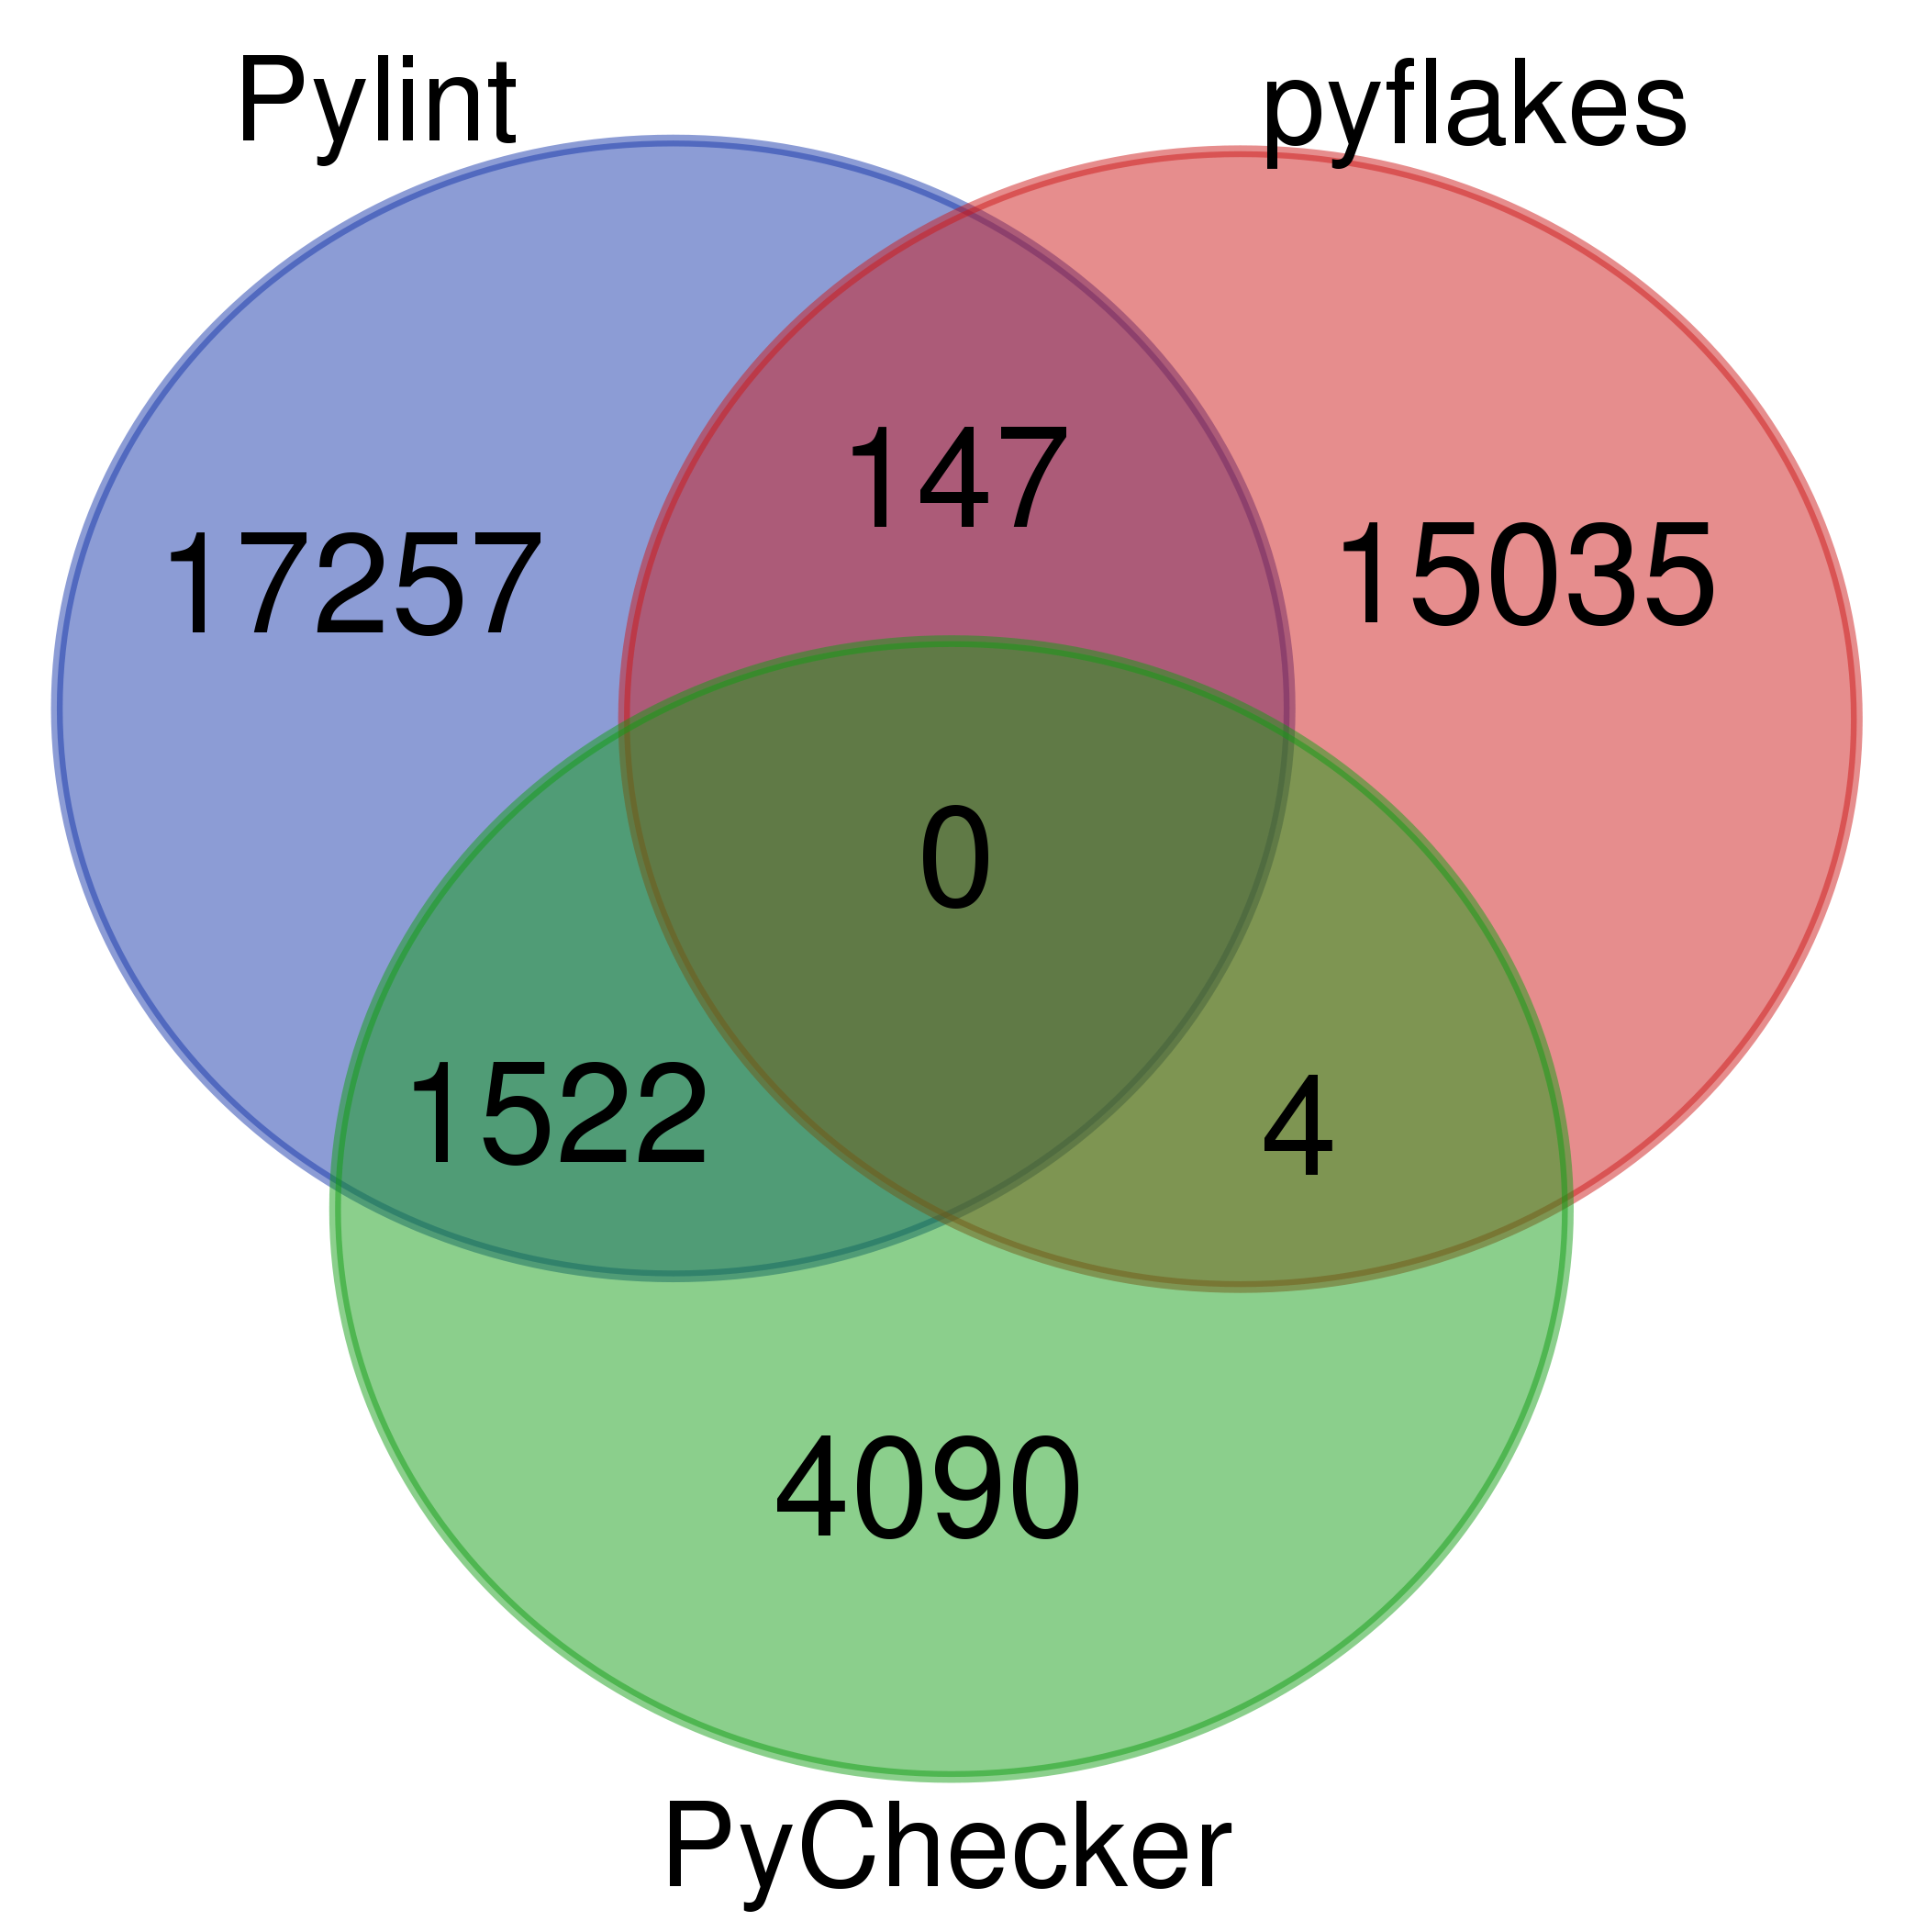
\includegraphics[width=0.35\columnwidth]{python.png}
  \caption{Mutants killed by Python static analysis tools.}
  \label{fig:pythonvenn}
\end{figure}

\begin{table}
  \begin{tabular}{l|r|r|r|r|r}
    & \multicolumn{2}{|c|}{Findings} & \multicolumn{2}{|c|}{Mutation Score}  & Mutant \\
    Tool & Mean & Median & Mean & Median & Ratio\\
    \hline
    \hline
    Pylint & 2.24 & 1.00 & 0.22 & 0.20 & 0.097 \\
    Clean (0) & - & - & - & - & - \\
    \hline
    pyflakes & 2.4 & 1.00 & 0.03 & 0.00 & 0.012 \\
    Clean (12) & - & - & 0.02 & 0.00 & - \\
    \hline
    PyChecker & 0.56& 0.00 & 0.10 & 0.00 &  0.183 \\
    Clean (21) & - & - & 0.01 & 0.00 \\
    \hline
  \end{tabular}
  \caption{Python tool results over all projects.}
  \label{tab:scorepython}
\end{table}


Figure \ref{fig:pythonvenn} shows the mutants killed by the Python analysis tools, and Table \ref{tab:scorepython} provides numeric results for projects and clean projects, respectively.

For {\bf RQ1}, Pylint and pyflakes both killed more than 15,000 mutants killed by no other tool; Pylint killed more mutants, but the relative difference was much smaller than in our Solidity or Java analysis.  It is clear both tools are well worth using, assuming these are not false positives.  Pyflakes' mutation score is lower than unique kills might suggest because it has almost no overlap with the other two tools.  It is doing something different.

The mutant ratios {\bf RQ2} suggest that PyChecker might be better than pyflakes, in fact, and better than Pylint, because while it killed fewer mutants, it also produced fewer findings by far, overall.  PyChecker would be a good choice for quick and dirty analysis of code on the fly, perhaps, in that it had excellent mutation scores for some programs (hence a high mean) but is relatively ``quiet'' compared to the other tools.  However, its very low median mutation score is troubling; it may simply not work for some code.  A combination of pyflakes and Pylint seems safer, though adding the relatively low-findings PyChecker seems likely to have little cost.  For Python, all of our measures are required to get a good picture.

\begin{figure}
  {\scriptsize
    % \begin{itemize}
    \raggedright
  \url{https://stackoverflow.com/questions/1428872/pylint-pychecker-or-pyflakes}\\
  \url{https://www.reddit.com/r/Python/comments/ii3gm/experience_with_pylint_pychecker_pyflakes/}\\
  \url{https://www.slant.co/versus/12630/12631/~pylint_vs_pyflakes}\\
  \url{https://news.ycombinator.com/item?id=12748885}\\
  \url{https://doughellmann.com/blog/2008/03/01/static-code-analizers-for-python/}\\
  %\end{itemize}
  }
\caption{Discussions of Python static analysis tools.}
\label{fig:blogpython}
\end{figure}

For {\bf RQ3}, there were again no academic comparisons we could find.  However, opinions on the web were quite common (see Figure \ref{fig:blogpython}, which lists ones we examined).  It is hard to summarize the overall opinion here, since it ranges considerably.  There is probably general agreement that PyChecker is old and maybe less useful, but also terse and sometimes helpful.  Pylint is the most recommended tool, and the general complaint that it is too picky was mitigated in our results by turning off clearly informative-only findings; users not configuring Pylint will probably see even more killed mutants, but likely a worse mutant ratio because mutants tend to introduce non-stylistic problems.  Pyflakes is also well liked, and supposedly less verbose than Pylint; we did not see this in our results, but that may be because we configured Pylint, and pyflakes aims to focus on ``actual bugs'' so it is equally verbose for mutants, which are likely to be actual bugs.
For {\bf RQ4} there were no clean projects for the known-to-be-aggressive Pylint.  Performance for the other two tools was worse on projects for which they were clean, again failing to support the possibility that our definition of killing a mutant is too restrictive.

For Python, as with Java, many mutants we inspected for {\bf RQ5} involved deletion of a call or change in comparison operator, leading to a likely method call or access to a variable containing {\tt None}, and the generated finding reported this problem.  Another example of a possibly engine-based mutation difference is that pyflakes did a much better job than the other tools of detecting cases where a mutant caused an exception to be unwisely ignored; these accounted for more than 10\% of differentially-relevant mutants.  We assume the issue is engine-based in that while pyflakes did by far the best at this (real) problem, there were instances where another tool found the problem and it did not.  On the other hand, pyflakes, in the sample we examined, did worst at detecting mutants that removed a needed argument from a function call, another common pattern (Pylint performed best for this type of mutant).  Again, based on a qualitative examination of many mutants, we believe the results to primarily rest on realistic faults, which some tools correctly detected and others did not.

\subsection{Threats to Validity}

The primary threat to validity in terms of generalization is that we only examined nine static analysis tools, and our analyses were restricted to 100 smart contracts, 15 Java projects, and 25 Python projects.   Because it is hard to identify a ground truth to compare with (the motivation for our approach), we cannot be certain that our rankings of tools are correct even for these tools and this code.  However, where there are existing discussions of the tools, our results seem to agree with these, but add substantial detail.

We used the Universal Mutator \cite{universalmutator,regexpMut}, which aggressively produces large numbers of mutants, but does not target any particular software defect patterns, to generate all mutants.
There is no room in the paper to present the exact set of projects analyzed, but we have provided an (anonymized) github repository containing raw results for inspection by reviewers, or further analysis by other researchers (\url{https://github.com/mutantsforstaticanalysis/rawdata}).
\section{Related Work}

The goal of ``analysing the program analyser'' \cite{cadar2016analysing} and applying better automated methods to evaluate and improve analysis tools has become recently more popular and, we suspect, more possible.  The irony of using mostly ad-hoc, manual methods to test and understand static analysis tools is apparent; however, the fundamentally incomplete and heuristic nature of effective analysis tools makes this a challenge similar to testing machine learning algorithms \cite{OnlyOracle}; most tools will not produce ``the right answer'' all the time, by their very nature.  This is a result of both algorithmic constraints and basic engineering trade-offs.  While comparisons of static analysis tools \cite{CompareJavaTools,durieux2019empirical, Parizi,slither,pashchenko2017delta} have appeared in the literature for years, these generally involved large human effort and resulting smaller scale, did not make a strong effort to address false positives, or restricted analysis to, e.g., a known defects set \cite{AllBugs, do2016toward}.  Known defect sets are particularly vulnerable to tools intentionally overfitting/gaming the benchmark; our approach makes it easy to compare tools on ``fresh'' code to avoid this risk.  Compared to well-known studies of Java tools \cite{AllBugs,CompareJavaTools} our approach used a larger set of subject programs (1.8 MLOC total vs. 170-350KLOC) and thousands of \emph{detected} (and tens of thousands of potential) faults, vs. e.g., about 500 known defects \cite{AllBugs}.  Results not using defect sets are even more limited in that humans can only realistically examine a few dozens of each type of warning \cite{CompareJavaTools}.

Cuoq et al. \cite{regehrRandom} proposed the generation of random programs (\emph{\'a la} Csmith \cite{csmith}) to test analysis tools aiming for soundness, in limited circumstances, but noted that na\"ive differential testing of analysis tools was not possible.  This paper proposes a non-na\"ive differential comparison (not, exactly, differential testing, however, in that only aggregate results are possible to interpret without human intelligence), based on the observation that the ability to detect program mutants offers an automatable way to tell which of two tools is better (for a given universe of examples, at least) at telling faulty from non-faulty code.

Klinger et al. propose a different approach to differential testing of analysis tools \cite{klinger2019differentially}.  Their approach is in some ways similar to ours, in that it takes as input a set of seed programs, and compares results across new versions generated from that seed.  The primary differences are that their seed programs must be warning-free (which greatly limits the set of input programs available) and their tool must parse and understand the programs, and that the new versions are based on adding new assertions, not ``breaking'' the original code.  We allow arbitrarily buggy seed programs (thus many more real programs can be used), and can, due to the any-language nature of the mutation generator we use, operate even in new languages without further development effort.  Further, their approach only identifies problems when tools are outliers compared to numerous other tools in either detecting a bug (precision) or not detecting it (soundness), and so requires comparing multiple tools.  Our approach has some utility for even a single tool (you can just examine prioritized un-detected mutants).  On the other hand, their approach can identify precision issues, while we offer no real help with false positives (in theory, you could apply their majority-vote method to mutants only a few tools flag, but mutants \emph{are} usually faults. in contrast to their introduction of checks that may be guaranteed to pass, so this is probably not very helpful).  Most importantly, however, their approach only applies to tools that check assertions, rather than more general, popular static analysis tools that only identify bad code patterns.

Finally, we essentially adopt the approach of the large body of work on using mutants in software testing \cite{jia2011analysis,demillo1978hints,budd1980theoretical, groce2015verified,groce2018verified,MutGoogle,ivankovic2018industrial,mutKernel}, but re-define killing a mutation for a static analysis context.
\section{Conclusions and Future Work}

In this paper, we showed that program mutants can be used as a proxy
for real faults, to compare (and motivate improvements to) static
analysis tools.  Mutants are attractive in that changing a mostly
correct program usually introduces a bug into it; this is the basis of
mutation testing, after all, and a large body of work supports the
claim that at least 60-70\% of mutants are fault-inducing.   This
means we can assume mutants are faulty, and escape the
ground-truth/false positive problem that makes comparing static
analysis tools so labor-intensive.  It cannot help with precision
problems, directly, but combined with finding counts for un-mutated
code, our approach can identify tools that detect mutants well,
adjusted for their general tendency to flag any code as faulty.  We
evaluated 9 popular static analysis tools, for Solidity smart contracts, Java,
and Python, and offer advice to users of these tools.  For Solidity,
academic research evaluations of the tools generally agreed strongly
with our conclusions, but lacked the detail mutant analysis contributed.
We were also able to use our methods, plus a novel mutant prioritization scheme, to
identify three useful new detectors for the Slither smart contract
analyzer.

As future work, we would like to further validate our approach and
improve our admittedly \emph{ad hoc} mutant distance metric.  Allowing
user feedback \cite{EndUserMistake,OnlyOracle}, or applying metric
learning methods \cite{kulis2012metric} (particularly unsupervised
learning \cite{scholkopf1998nonlinear,tipping1999probabilistic}) are
the most obvious and interesting possibilites for a better metric.
Finally, mutant prioritization should be applicable to improving
software testing, as well \cite{groce2018verified}.

\bibliographystyle{plain}
\bibliography{bibliography,bibliography_ag,rahul}

\end{document}
